\documentclass[11pt]{article}
\usepackage{zpj}
\usepackage{braket}
\usepackage{amssymb}
\begin{document}
\title{Hadamard gate with $(u/2h)^2\in \mathbb{N^+}$}
\author{Peijun Zhu}
\maketitle

\section{Solution to Hamiltonian}
Consider Hamiltonian $H=\omega\hat  N+ub^\dagger b+h\hat N(b^\dagger+b)$, it is obvious $[H, \hat N]=0$ so that we are able to diagonalize $H$ and $\hat N$ at the same time. We look for eigenstate $\ket{n, m}=\ket{n}\otimes\ket{\varphi_m}$. In the subspace of $\ket{n}$,
\begin{align}
H&=\omega n+ub^\dagger b+hn(b^\dagger+b)\\
&=u\tilde b^\dagger\tilde b+\omega n-\frac{h^2n^2}{u}, \quad\tilde b=b+\frac{hn}{u}
\end{align}
The $\tilde b^\dagger$ is displaced creation operator. Eigenstates of $\tilde b^\dagger\tilde b$ are $D(-hn/u)\ket{m}$ because
\begin{equation}\tilde b^\dagger\tilde b \big[D\ket{m}\big]=DD^\dagger\tilde b^\dagger\tilde b D\ket{m}=Db^\dagger b\ket{m}=m\big[D\ket{m}\big]\end{equation}
The energy spectrum is:
\begin{equation}E_{n, m}=um+\omega n-\frac{h^2n^2}{u}, \quad \ket{n, m}=\ket{n}\otimes D(-hn/u)\ket{m} \end{equation}

\section{Time evolution}
For arbitrary initial state $\ket{\psi}$ we can plug in $\sum_n \ket{n}\bra{n}$ to write it as $\sum_n c_n \ket{n}\otimes \ket{\varphi_n}$. Its time development is

\begin{equation}\ket{\psi(t)}=\sum_n c_n\exp(\ii n^2h^2t/u)\ket{n(t)}\otimes\exp(-\ii u\tilde{b}^\dagger\tilde{b}t)\ket{\varphi_n} \end{equation}
We have phase factors
\begin{equation}\phi_1=\frac{n^2h^2}{u}t, \quad\phi_2=-u\hat n_b t\end{equation}
for system $A$ and $B$ respectively. The $\phi_2$ is complicated because $\hat n_b = \tilde b^\dagger\tilde b$ depends on the displacement operator $D(-hn/u)$.

\section{Choice of parameters}
\begin{itemize}
\item We want to make first phase factor $\phi_1=n^2\pi/2$, which gives
\begin{equation}
t=\frac{\pi u}{2h^2}
\end{equation}
At the same time, $\phi_2=- (u/h)^2n_b\pi/2$

\item To kill the complicated $\phi_2\propto\hat n_b$ term, we want to make $\phi_2/2\pi=-\hat n_b(u/2h)^2$ have integral eigenvalues, which requires
\begin{equation}
	l\mdef\left(\frac{u}{2h}\right)^2\in \mathbb{N^+}\label{int}
\end{equation}
\end{itemize}
With these parameters of Hamiltonian and time, if we start with product state, we will end up with cat state. 
\begin{equation}
\ket{\alpha}\otimes\ket{\varphi}\rightarrow \ket{\mathrm{cat}}\otimes \ket{\varphi}
\end{equation}
We can also rewrite
\begin{equation}
t=\frac{2\pi}{u}l\label{time}
\end{equation}
During time evolution, $b$ system goes back to pure state with period
\begin{equation}T = \frac{2\pi}{u}\end{equation}
\paragraph{Conclusion} (\ref{int}) and (\ref{time}) are two conditions to make a Hadamard gate. $l$ determines how many cycles $b$ mode rotates during time evolution. 

As a special case, if $u/h$ is integer, it should be even. For $u/h=6$ (or $l=9$), the video \url{https://www.youtube.com/watch?v=tAXxqMaHJJA} shows 9 cycles of $b$ mode. For non-integer $l$, the deviation from cat state is shown in Fig.~\ref{l}
\begin{figure}[htbp!]
\centering
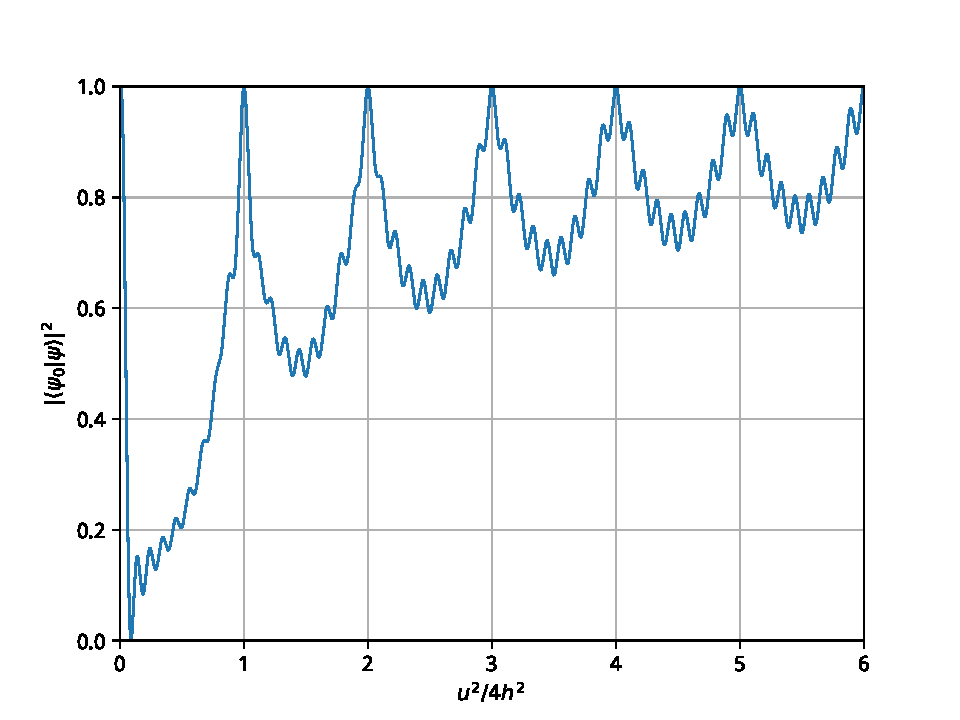
\includegraphics[width=\textwidth]{fidelity.pdf}
\caption{Overlapping between $\ket{\psi(t)}$ and ideal two cat state $\ket{\psi_0}=\ket{\mathrm{cat}}\otimes\ket{0}$}\label{l}
\end{figure}
\end{document}